\chapter{Objetivos del proyecto\label{03analisisObjetivos}}

Este proyecto pretende extender la funcionalidad del lenguaje Deimos a través de una librería de Java, que permita a los desarrolladores crear sus propios propios conjuntos variables de datos, generar estos datos a través de datos propios o autogenerados, crear conjuntos de datos pseudoaleatorios que se puedan replicar y exportar estos datos a una base de datos final NoSQL automáticamente, a un fichero en formato JSON, CSV o TXT o simplemente imprimir el resultado por consola.

A través de una librería y un fichero Deimos para la especificación de generaciones de datos NoSQL, el usuario podrá definir qué reglas contendrán los datos finales, su generación y los datos de entrada a través de ficheros o por consultas directas a bases de datos y por último la salida de estos datos.

\section{El lenguaje Deimos}

La especificación Deimos consta de tres partes fundamentales como se describe en~\cite{deimosAlberto}.

\begin{enumerate}
	\item \emph{Entrada de datos}: Deimos proporciona la entrada de datos de fuentes externas para que el generador posteriormente seleccione y modifique estos datos pseudoaleatoriamente en vez de generarlos. Se encuentran los 5 siguientes tipos de entradas de datos:
	\begin{itemize}
		\item \emph{Fichero de texto}: Debe estar separados por saltos de linea, cada linea se considera un dato distinto.
		\item \emph{Json}: El fichero Json debe contener un array de datos.
		\item \emph{CSV}: Se podrá definir en el módulo de la entrada de datos un mapeo de las columnas para la representación de las mismas en las reglas del generador.
		\item \emph{Base de datos}: Podrá ser de tipo SQL o MongoDB, se proporcionará una cadena con la conexión a la misma (puede ser local o externa) junto con al query que se quiere realizar de la misma, al igual que en el fichero CSV se podrán mapear las columnas dela petición con una clave.
		\item \emph{Ejecutable Python}: También se acepta la entrada de lenguaje código Python para ser ejecutado por el programa y utilizar la salida del mismo como entrada de datos de generación.
	\end{itemize}
	
	Cada entrada de datos tiene tres valores más por definir:
	
	\begin{itemize}
		\item \emph{Orden}: Puede ser aleatorio o en orden, por defecto es aleatorio.
		\item \emph{Ciclo}: Repetitivo o de un solo recorrido, si se establece `once' como ciclo una vez se acaben los datos de la entrada se generarán valores nulos que podrán o no ser modificados posteriormente.
		\item \emph{Valor por defecto}: Valor que se muestra finalmente si la generación ha resultado nula.
	\end{itemize}

	Para construir correctamente las cadenas de conexión y queries para la entrada de valores por bases de datos se deberá utilizar el siguiente patrón:

	\textbf{Entrada de datos BD relacionales}:

	\begin{figure}[H]
		\centerline{\emph{jdbc:Tipo de SGDB://IP:Puerto/Schema?user=Username\&password=Contraseña/Query}}
	\end{figure}

\begin{longtable}{|l|l|}
	\hline
	\textbf{Nombre}      & \textbf{SchemaName} \\ \hline
	\endfirsthead
	%
	\multicolumn{2}{c}%
	{{\bfseries Table \thetable\ continued from previous page}} \\
	\hline
	\textbf{Nombre}      & \textbf{SchemaName} \\ \hline
	\endhead
	%
	MySQL                & mysql                                         \\ \hline
	MariaDB              & mariadb                                       \\ \hline
	Oracle               & oracle:thin                                   \\ \hline
	Microsoft SQL Server & sqkserver                                     \\ \hline
	PostgreSQL           & postgreSQL                                    \\ \hline
	IBM DB2 						 & db2 {[}:net\textbackslash{}|:ibmdb\textbackslash{}|:ids{]} \\ \hline
	Elastic Search       & es                                            \\ \hline
	SQLite               & sqlite                                        \\ \hline
	Microsoft Access     & ucanaccess                                    \\ \hline
	\caption{Bases de datos relacionales para entrada de datos}
	\label{tab:bbss_input_SQL}\\
	\end{longtable}

	\textbf{Entrada de datos BD MongoDB}:

	\begin{figure}[H]
		\centerline{\emph{mongodb://IP:Puerto/BBDD.Coleccion/Query}}
	\end{figure}


	Esta sección también alberga la semilla (seed) de la generación de números pseudo-aleatorios

	\item \emph{Salida de datos}: Al igual que con la entrada, Deimos proporciona varios tipos de salida de datos hacia fuentes externas. Hay 3 tipos de outputs:
	\begin{itemize}
		\item \emph{Consola}: Las entidades generadas se muestran por consola.
		\item \emph{folder}: Crea un fichero de un formato predeterminado y escribe en él las entidades generadas, si el fichero no existe lo crea y si existe remplaza su contenido. Los formatos de salida disponible son `TXT', `CSV', `JSON'.
		\item \emph{Database}: Guarda los datos generados en una base de datos con la cadena de conexión proporcionada que se indicó anteriormente. Si el esquema o colección ya existía se deben agregar los nuevos elementos pero nunca sobrescribir su antiguo contenido.
	\end{itemize}
	
	\item \emph{Reglas para la generación de los datos}: Define las reglas para los atributos que definen las entidades, las reglas poseen un identificador de la regla, un tipo de la misma y un conjunto de modificadores. Entre los tipos podemos destacar los siguientes:

	\begin{itemize}
		\item Primitivos: Aquí se encuentran los datos básicos, cadena, booleano, número entero, número decimal y fechas.
		\item variación: Tipo de datos variables.
		\item Identificadores de identidad: atributos que definen una variable.
		\item atributos de colección: Listas, mapas, tuplas y conjuntos de datos no definidos.
		\item Referencia: Tipo que referencia el identificador de otra entidad de la generación.
	\end{itemize}

	Los modificadores son propiedades capaces de generar un valor (modificador src extrae un valor de un input, range crea un valor entre dos preestablecidos, pattern genera un dato que cumple una cierta expresión regular), modificarlo (fixed proporciona un valor por defecto cuando el valor que se va a devolver es nulo, fixedPrecision modifica los decimales de los datos de tipo float) o generar uno nuevo sin importar el de entrada (null genera un nulo dada una probabilidad, strange crea un dato de un tipo distinto al del atributo con una probabilidad).
\end{enumerate}


\subsection{Sintaxis de la especificación Deimos\label{03Deimos}}

En cuanto a la sintaxis podemos afirmar que Deimos prevee un sintaxis permisiva. Esto quiere decir que si se encuentran errores en alguna de sus reglas, simplemente esta pasará a la siguiente omitiéndola. Utiliza una sintaxis sencilla, sin apenas separadores, y utilizando palabras claves para identificar los distintos apartados (`Input', `Output', `Rules') como los atributos, las reglas, sus modificadores, etc. También utiliza delimitadores de código para separar clave y valor `:'; valores encapsulados `()' y `\{\}'; para representar rangos `[]' y para representar cadenas `\"'. Además de las palabras y los caracteres reservados, se utilizan variables que sirven para que el usuario represente el valor que va a guardar.

\begin{figure}[h!]
	\centerline{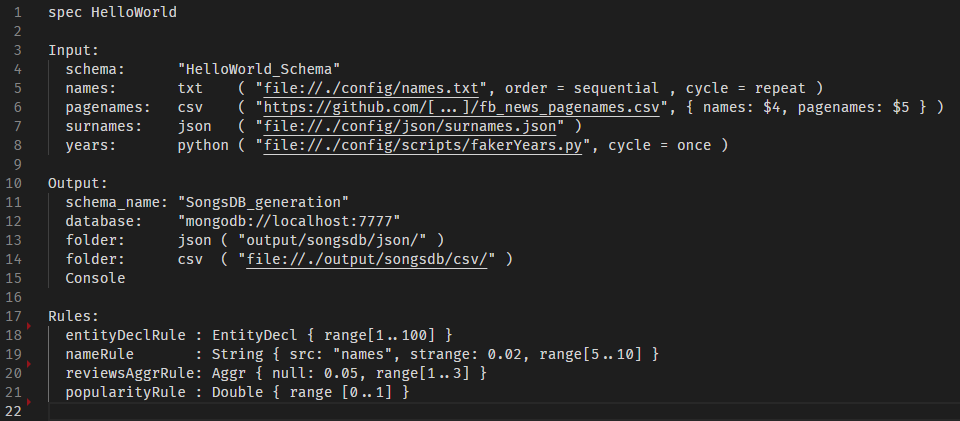
\includegraphics[width=1\textwidth]{Ejemplo_deimos.png}}
	\caption{Ejemplo sencillo de fichero Deimos.}
	\label{figure:deimosexample}
\end{figure}

En la figura \ref{figure:deimosexample} se puede ver un ejemplo con una definición de los tres apartados de un script Deimos. En el Input podemos apreciar 4 entradas de datos procedentes de un fichero txt, json y csv y de un programa ejecutable Python. A estas entradas se les ha establecido un orden y un ciclo y un identificador propio para poder referenciarlas desde las reglas. En el apartado de las salidas vemos 3 módulos distintos, la salida por consola, y las salidas a los ficheros json y csv en la carpeta output/songsdb. Por último el apartado de las reglas vemos 4 reglas distintas cada una con un tipo determinado EntityDecl (declaración de entidad, asocia un atributo de tipo ID para poder identificarlo unívocamente), String, Aggr u Double las cuales tienen además distintos modificadores range, src, null, etc.

% \subsection{Arquitectura del lenguaje}

% Deimos ha sido construido con Xtext~\cite{efftinge_spoenemann}, un framework construido en Java para diseñar lenguajes de programación y lenguajes de dominio específico. 

% Xtext proporciona además herramientas para parsear, linkar, validar y compilar los documentos. Es por esto que nuestro generador utiliza una clase generada por Xtext capaz de leer un documento y devolverlo en forma de objeto para su uso, convirtiendo a los diferentes tipos del lenguaje Java cada uno de los atributos especificados.




%%% Local variables:
%%% TeX-master: "memoria.tex"
%%% coding: utf-8
%%% ispell-local-dictionary: "spanish"
%%% TeX-parse-self: t
%%% TeX-auto-save: t
%%% fill-column: 75
%%% End:
